% Figure from MATH 591 notes, section 66 (Lecture 22).
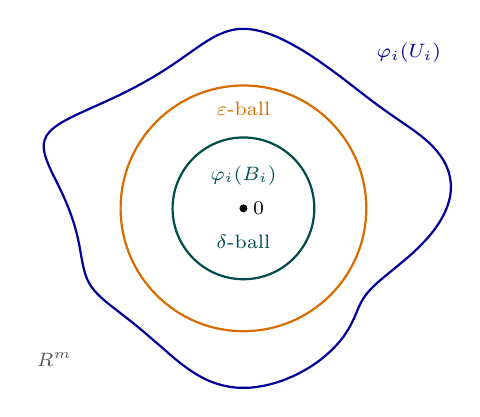
\begin{tikzpicture}[scale=1.2]
\draw[blue!60!black, thick] plot[smooth cycle] coordinates {(2.150,0.000) (2.188,0.132) (2.195,0.260) (2.173,0.381) (2.126,0.493) (2.058,0.593) (1.976,0.683) (1.884,0.763) (1.787,0.836) (1.689,0.904) (1.590,0.972) (1.490,1.042) (1.386,1.118) (1.278,1.200) (1.162,1.290) (1.038,1.386) (0.904,1.484) (0.764,1.583) (0.619,1.676) (0.473,1.758) (0.330,1.825) (0.192,1.872) (0.062,1.897) (-0.060,1.897) (-0.176,1.872) (-0.290,1.825) (-0.405,1.758) (-0.526,1.676) (-0.658,1.583) (-0.804,1.484) (-0.962,1.386) (-1.133,1.290) (-1.310,1.200) (-1.487,1.118) (-1.655,1.042) (-1.806,0.972) (-1.932,0.904) (-2.026,0.836) (-2.087,0.763) (-2.113,0.683) (-2.107,0.593) (-2.076,0.493) (-2.027,0.381) (-1.967,0.260) (-1.906,0.132) (-1.850,0.000) (-1.803,-0.132) (-1.766,-0.260) (-1.739,-0.381) (-1.719,-0.493) (-1.700,-0.593) (-1.678,-0.683) (-1.648,-0.763) (-1.605,-0.836) (-1.547,-0.904) (-1.474,-0.972) (-1.388,-1.042) (-1.290,-1.118) (-1.185,-1.200) (-1.075,-1.290) (-0.963,-1.386) (-0.849,-1.484) (-0.735,-1.583) (-0.617,-1.676) (-0.495,-1.758) (-0.365,-1.825) (-0.226,-1.872) (-0.078,-1.897) (0.079,-1.897) (0.242,-1.872) (0.405,-1.825) (0.563,-1.758) (0.710,-1.676) (0.840,-1.583) (0.950,-1.484) (1.038,-1.386) (1.104,-1.290) (1.153,-1.200) (1.190,-1.118) (1.222,-1.042) (1.258,-0.972) (1.304,-0.904) (1.366,-0.836) (1.445,-0.763) (1.541,-0.683) (1.651,-0.593) (1.769,-0.493) (1.886,-0.381) (1.994,-0.260) (2.084,-0.132)};
\node[blue!60!black, font=\scriptsize] at (1.75,1.65) {$\varphi_i(U_i)$};
\draw[orange!85!black, thick] (0,0) circle (1.3); \node[orange!85!black, font=\scriptsize] at (0,1.05) {$\varepsilon$-ball};
\draw[teal!60!black, thick] (0,0) circle (0.75); \node[teal!60!black, font=\scriptsize] at (0,0.35) {$\varphi_i(B_i)$};
\node[teal!60!black, font=\scriptsize] at (0,-0.35) {$\delta$-ball};
\fill (0,0) circle (1.2pt) node[right, font=\scriptsize] {$0$};
\node[font=\scriptsize, gray!70!black] at (-2.0,-1.6) {$\mathbb{R}^m$};
\end{tikzpicture}
